%% LyX 2.3.4.4 created this file.  For more info, see http://www.lyx.org/.
%% Do not edit unless you really know what you are doing.
\documentclass[british]{beamer}
\usepackage{mathptmx}
\usepackage[T1]{fontenc}
\usepackage[latin9]{inputenc}
\usepackage{babel}
\usepackage{algorithm2e}
\usepackage{amstext}
\usepackage{amssymb}
\usepackage{graphicx}
\ifx\hypersetup\undefined
  \AtBeginDocument{%
    \hypersetup{unicode=true}
  }
\else
  \hypersetup{unicode=true}
\fi

\makeatletter
%%%%%%%%%%%%%%%%%%%%%%%%%%%%%% Textclass specific LaTeX commands.
% this default might be overridden by plain title style
\newcommand\makebeamertitle{\frame{\maketitle}}%
% (ERT) argument for the TOC
\AtBeginDocument{%
  \let\origtableofcontents=\tableofcontents
  \def\tableofcontents{\@ifnextchar[{\origtableofcontents}{\gobbletableofcontents}}
  \def\gobbletableofcontents#1{\origtableofcontents}
}

%%%%%%%%%%%%%%%%%%%%%%%%%%%%%% User specified LaTeX commands.
\DeclareMathAlphabet{\mathcal}{OMS}{cmsy}{m}{n}
\usetheme[oldstylearrows,nologo,numbers,algorists]{CIMAT}

% or ...

\setbeamercovered{transparent}
% or whatever (possibly just delete it)
\usepackage[euler-digits]{eulervm}
\usefonttheme{professionalfonts}
\usepackage{dsfont}
%\usepackage[table]{xcolor}
%\usepackage{booktabs}

%\usepackage[usenames,dvipsnames]{xcolor}
\usepackage{tcolorbox}
\usepackage{tabularx}
\usepackage{array}
\usepackage{colortbl}
\tcbuselibrary{skins,fitting}

\newcolumntype{Y}{>{\raggedleft\arraybackslash}X}

\DeclareMathOperator{\posdef}{+def}
\DeclareMathOperator{\tr}{tr}
\DeclareMathOperator{\cov}{cov}
\DeclareMathOperator{\variance}{var}
\DeclareMathOperator{\lcp}{lcp}
\renewcommand{\mathbf}{\boldsymbol}
\DeclareMathOperator{\idv}{div}
\DeclareMathOperator{\diag}{diag}

\SetKwInOut{Input}{Input}
\SetKwInOut{Output}{Output}
\SetKwInOut{Data}{Parameters}
\SetKwInOut{Result}{output}
\SetKw{struct}{struct}
\SetKw{KwTo}{to}
\SetKw{Throw}{throw}
\SetKw{KwRet}{return}
\SetKw{Return}{return}
\SetKwProg{Function}{function}{:}{end}
\SetKwProg{lFunction}{function}{}{}
\SetKwBlock{Begin}{begin}{end}
\SetKwRepeat{Repeat}{repeat}{until}
\SetKwIF{If}{ElseIf}{Else}{if}{then}{else if}{else:}{end}
\SetKwSwitch{Switch}{Case}{Other}{select}{for}{case}{otherwise}{end}{end}
\usepackage{algpseudocode}
\SetKwFor{For}{for}{do:}{end}
\SetKwFor{ForPar}{parallel for}{do:}{end}
\SetKwFor{ForEach}{for each}{do:}{end}
\SetKwFor{ForAll}{for all}{do:}{end}
\SetKwFor{While}{while}{do:}{end}

\SetKw{Static}{static}
\SetKw{Const}{const}
\SetKw{Struct}{struct}
\SetKw{Class}{class}
\SetKw{New}{new}
\SetKw{Delete}{delete}
\SetKw{Char}{char}
\SetKw{Integer}{int}
\SetKw{Long}{long}
\SetKw{Unsigned}{unsigned}
\SetKw{Signed}{signed}
\SetKw{Boolean}{bool}
\SetKw{KwNot}{not}
\SetKw{KwAnd}{and}
\SetKw{KwOr}{or}
\SetKw{KwXor}{xor}

\SetKwFunction{node}{node}
\SetKwFunction{sort}{std::sort}
\SetKwFunction{lcp}{lcp}
\SetKwFunction{strlen}{strlen}
\SetKwFunction{strcmp}{strcmp}
\SetKwFunction{fibonacci}{fibonacci}
\SetKwFunction{pushback}{push-back}
\SetKwFunction{alphanumeric}{to-alpha}
\SetKwFunction{back}{back}
\SetKwFunction{neighborhood}{neighborhood}
\SetKwFunction{buildsuffix}{build-suffix-array}
\SetKwFunction{isEmpty}{is-empty}
\SetKwFunction{isNull}{is-null}
\SetKwFunction{isBetter}{can-improve}
\SetKwFunction{isUnvisited}{is-unvisited}
\SetKwFunction{isValid}{is-valid}
\SetKwFunction{improve}{visit-or-improve}
\SetKwFunction{mycomparator}{cmp}

\SetKwFunction{trie}{trie}
\SetKwFunction{map}{std::map}
\SetKwFunction{addword}{add-word}
\SetKwFunction{findword}{find-word}
\SetKwFunction{isEmpty}{is-empty}
\SetKwFunction{isNull}{is-null}

\SetSideCommentRight

\newcolumntype{Y}{>{\raggedleft\arraybackslash}X}

\tcbset{smallvalues/.style={enhanced,fonttitle=\bfseries,fontupper=\normalsize\sffamily,
colback=zorange!10!white,colframe=zorange!90!black,colbacktitle=zorange!90!white,
coltitle=white,center title}}

\makeatother

\begin{document}
\title[Dynamic Programming]{Dynamic Programming}
\author[Ulises Tirado Zatarain]{Ulises Tirado Zatarain~  \inst{1}\\
(ulises.tirado@cimat.mx) }
\institute[Algorists]{\inst{1}Algorists Group}
\date[Nov, 2020]{November, 2020}

\makebeamertitle
\pgfdeclareimage[height=0.75cm]{algorists}{algorists.png}
\logo{\pgfuseimage{algorists}}

\AtBeginSubsection[]{
  \frame<beamer>{ 
    \frametitle{Outline}   
    \tableofcontents[currentsection,currentsubsection] 
  }
}

%\beamerdefaultoverlayspecification{<+->}
\begin{frame}{Outline}

\tableofcontents{}

\end{frame}

\section{Introduction}

\subsection[Definitions]{Definitions}
\begin{frame}{What is dynamic programming?}

\begin{definition}[Dynamic Programming]
 It's a technique for mathematical programming (optimization), or
in other words, a paradigm to problem solving. So, the word ``programming''
is not directly meaning a computer program or an algorithm. The actual
meaning is more similar to linear programming or planning or taking
decisions.
\end{definition}

\begin{itemize}
\item It consists in:

\begin{itemize}
\item Split the problem in smaller sub-problems:
\begin{itemize}
\item recurrence relationship
\item optimal sub-structure
\end{itemize}
\item We stop when have a trivial problems (base cases)
\item Store smaller solutions (memoization, states) 
\item Merge the solutions when is need it
\item Difference with D\&C: \textbf{overlapping and compute a value}
\end{itemize}
\end{itemize}
\end{frame}


\subsection{A particular problem}
\begin{frame}{Recurrence relationship and tree of calls}

\visible<1->{Fibonacci sequence ($0,1,1,2,3,5,\ldots$) is the simplest
examples}

\begin{center}
\visible<2->{$F(n)=\begin{cases}
1 & n=1\\
F(n-1)+F(n-2) & n>1\\
0 & \textrm{otherwise}
\end{cases}$}
\par\end{center}

\begin{center}
\visible<3->{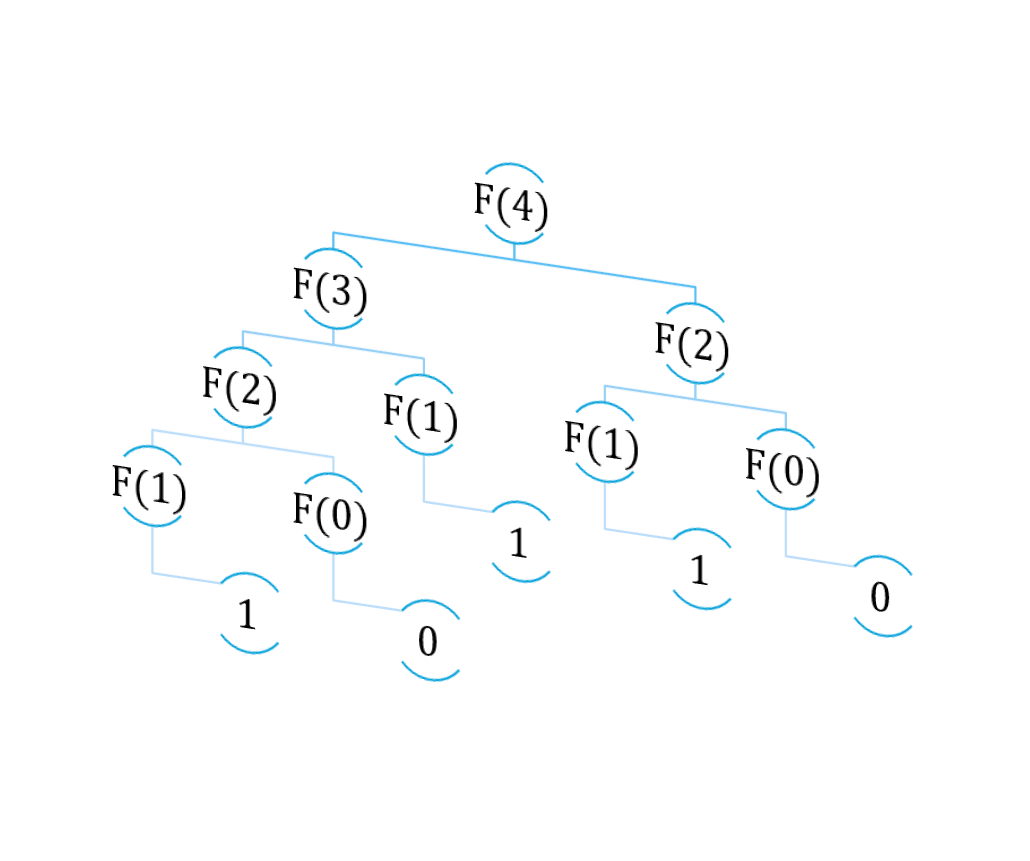
\includegraphics[viewport=47.9612bp 86.3415bp 446.039bp 340.569bp,clip,scale=0.5]{figures/fibonacci-tree}}
\par\end{center}

\end{frame}


\appendix

\section*{Appendix}

\subsection*{References}
\begin{frame}[allowframebreaks]{References}

\beamertemplatebookbibitems
\begin{itemize}
\item Introduction to Algorithms, Thomas H. Cormen
\item \href{https://github.com/Gansito144/algorists/tree/master/talks/dynamic_programming}{Algorists: Github Repository}
\item \href{https://en.wikipedia.org/wiki/Dynamic_programming}{Wikipedia: Dynamic Programming}
\item \href{https://www.hackerrank.com}{HackerRank}
\item \href{https://codeforces.com}{CodeForces}
\item \href{https://omegaup.com}{OmegaUp}
\item \href{https://leetcode.com}{LeetCode}
\end{itemize}
\end{frame}

\end{document}
